\subsection{Protocols}

	\par{The different building blocks of a network presented above allow for the transportation of information, but is is the use of protocols which provide the semantics. For a message to be decoded the parties involved must agree on some sort of well-defined syntax, so that noise can be separated from meaningul information, this is precisely the role of the various network protocols existing at all levels within a network.}

	\defn{PDU}{stands for protocol data unit, and is the basic unit	of information for any given protocol}

	\par{PDUs can be textual where rules of syntax and grammar are used to implement behaviour (e.g. HTTP), or binary where similar appropriate rules are used (e.g. TCP/IP). It is the role of PDUs to define what messages are legal to send, but is up to protocol semantics to define when to send them and what should be expected in response}

\subsubsection{Layers}

	\par{Communication systems are tipically organised into layers, which reduces complexity at each layer's level. Peers on the same layer, use that layer's protocol to communicate using services provided by the well-defined interfaces of the lower layers}

	\defn{OSI Model}{stands for \ita{Open Systems Interconnection Model} and is a conceptual model that characterises and standardises the communication functions of a telecommunication or computing system without regard to its underlying internal structure and technology. }

	\par{A design tool used widely to model layered communication channels is the \ita{OSI model}. It is merely a design tool, real implementations are more complex and usually the boundaries between layers are not so well defined.}

	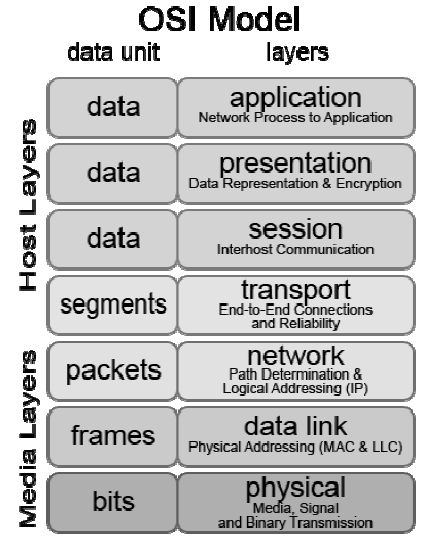
\includegraphics{osi.png}


